\documentclass{article}

\usepackage{arxiv}
\usepackage[utf8]{inputenc}
\usepackage[T1]{fontenc}
\usepackage{hyperref}
\usepackage{url}
\usepackage{booktabs}
\usepackage{amsmath,amssymb}
\usepackage{microtype}
\usepackage{graphicx}
\usepackage{natbib}
\usepackage{xcolor}
\usepackage{tabularx}
\usepackage{cleveref}

% ---------------------------------------------------------------- team settings
\newcommand{\RepoURL}{\url{https://github.com/canalesuva/DS6050-UVA-Project1}}
\newcommand{\TODO}[1]{\textcolor{red}{[TODO: #1]}}

% Results produced by code/run_experiments.py are picked up automatically.
\newcommand{\pending}[1]{\fbox{\parbox{0.92\linewidth}{\centering\small\textit{#1}}}}
\IfFileExists{results/numbers.tex}{\newcommand{\NTest}{1,560}
\newcommand{\HumanGap}{-0.64}
}{}

\title{Does the Scorer Widen the Gap? Socioeconomic Fairness of Neural Automated Essay Scoring for Students Served by Title~I}

\author{
  Carlos Canales \\ School of Data Science, University of Virginia
  \And
  \TODO{Teammate 2} \\ School of Data Science, University of Virginia
  \And
  \TODO{Teammate 3} \\ School of Data Science, University of Virginia
}

\renewcommand{\shorttitle}{SES Fairness in Neural Essay Scoring}

\begin{document}
\maketitle

\begin{abstract}
Automated essay scoring (AES) is moving into classrooms and state assessments, and the students most exposed to its errors are often those in high-poverty schools served by Title~I. Prior work on the PERSUADE corpus found that economic status is the demographic attribute most frequently associated with AES bias, yet it rarely separates the score gap already present in human ratings from the gap a model adds, and it seldom tests mitigation aimed at socioeconomic status (SES). We study 25{,}996 grade 6--12 argumentative essays from the public PERSUADE~2.0 corpus, of which about 80\% carry a flag for eligibility for federal assistance programs. We compare feature-based baselines with a fine-tuned DeBERTa-v3 regressor and measure fairness as the difference in signed prediction error between economically disadvantaged and non-disadvantaged students, overall and conditional on the human score. We then plan input ablations to locate the source of any bias (surface form versus content) and evaluate adversarial and reweighting-based mitigation, reporting the accuracy cost of each. Code and splits are public.
\end{abstract}

% =====================================================================
\section{Introduction}
\label{sec:intro}

Title~I of the Elementary and Secondary Education Act directs federal funding to schools with high concentrations of students from low-income families. These schools often have the largest class sizes and the least teacher time per essay, which makes them natural candidates for automated essay scoring (AES). The same students, however, are the ones a biased scorer would hurt most: a model that systematically under-scores economically disadvantaged writers turns a tool meant to save teacher time into one that compounds an existing achievement gap.

Human scores already differ by SES. On the PERSUADE corpus, higher-SES students score roughly two-thirds of a point higher on a 1--6 scale, and most of that gap is attributable to essay content rather than to how raters evaluate it \citep{kunievsky2026content}. A fair AES model should reproduce human judgments with \emph{equal error} across groups; it should not add a further gap on top. The question that matters for deployment is therefore not ``do predicted scores differ by SES?'' (they should, if human scores do) but ``conditional on the human score, does the model err in a direction that disadvantages one group?''

\paragraph{Research questions.}
\begin{itemize}
  \item[\textbf{RQ1}] \textbf{Amplification.} Do neural AES models produce larger or more negatively signed errors for economically disadvantaged students than for their peers, overall and at each human score level?
  \item[\textbf{RQ2}] \textbf{Mechanism.} Is any such bias driven by surface form (length, spelling, mechanics) or by content? We test this with controlled input ablations.
  \item[\textbf{RQ3}] \textbf{Mitigation.} How much of the gap can adversarial debiasing or group reweighting remove, and at what cost in accuracy (quadratic weighted kappa, QWK)?
\end{itemize}

\paragraph{Scope note.} PERSUADE records \emph{student-level} eligibility for federal assistance, not school-level Title~I status. We therefore study economically disadvantaged students, the population Title~I is designed to serve, and avoid claims about Title~I schools as institutions.

% =====================================================================
\section{Related Work}
\label{sec:related}

\paragraph{Neural AES.} Neural scorers replaced feature engineering with learned representations, beginning with recurrent models \citep{taghipour2016neural}. Pre-trained transformers now dominate; DeBERTa-v3 \citep{he2023debertav3} is a strong encoder for long-form regression, and long-context variants such as Longformer \citep{beltagy2020longformer} address the 512-token limit that truncates many student essays.

\paragraph{Fairness in AES.} \citet{loukina2019fairness} distinguish outcome fairness (equal score distributions) from error fairness (equal accuracy and equal signed error), arguing that the latter is the appropriate target when human scores themselves differ by group. \citet{litman2021fairness} found that different AES model families exhibit different biases across gender, race, and SES on elementary-school text-evidence essays.

\paragraph{Fairness on PERSUADE.} PERSUADE~1.0 and 2.0 \citep{crossley2022persuade,crossley2024persuade} were released partly to enable bias audits, pairing essays with demographic metadata. \citet{yang2024tapestry} evaluated nine AES methods on the corpus and found that economic status is the attribute most frequently associated with predictive bias, that prompt-specific models are more biased than cross-prompt ones, and that a feature-based SVM was competitive with neural models on both accuracy and fairness. \citet{kwako2024guess} reported that a fine-tuned XLNet scorer favored female over male and White over Black students, and that its hidden states weakly encoded demographic membership. \citet{yang2025prompt} extended the analysis to prompt-based GPT-4o scoring, showing that the model can partly infer first-language background and that bias is larger when it does.

\paragraph{Gap.} These studies \emph{measure} bias, mostly through aggregate group differences. Three questions remain open and motivate this project: (i) separating the model's added error from the human-score gap by conditioning on the human score; (ii) identifying whether SES bias flows through surface form or content; and (iii) testing mitigation methods targeted at SES, such as adversarial training with gradient reversal \citep{ganin2016domain,zhang2018mitigating}, on modern encoders.

% =====================================================================
\section{Dataset}
\label{sec:data}

\paragraph{Source and version.} We use PERSUADE~2.0 \citep{crossley2024persuade}, released under CC~BY~4.0.
\begin{itemize}\raggedright
  \item URL: \url{https://github.com/scrosseye/persuade_corpus_2.0}
  \item Version pin: \texttt{persuade\_corpus\_2.0\_train.csv}, Google Drive id \texttt{13phHyDzIsb0MHyJr6q-B-qIa9P2tM135}, last modified 2024-11-14, 616{,}894{,}963 bytes.
\end{itemize}

\paragraph{Contents.} The corpus contains 25{,}996 argumentative essays written by U.S.\ students in grades 6--12 in response to 15 prompts across two tasks (independent and source-based writing). Each essay has an adjudicated holistic score from 1 to 6 and writer metadata: gender, race/ethnicity, English-learner status, disability status (IEP or 504 plan), and economic disadvantage, defined by eligibility for federal assistance programs. Roughly 80\% of essays carry the economic-disadvantage flag. The raw file has one row per discourse element; we deduplicate to one row per essay.

\paragraph{Splits.} We hold out the password-protected official test file and create our own 80/10/10 train/validation/test split from the training file, stratified by prompt $\times$ score with seed 42. Essays without an SES flag are used for training but excluded from fairness metrics. \Cref{tab:data} summarizes the groups.

\begin{table}[h]
  \centering
  \caption{Holistic scores and essay length by economic-disadvantage status (full deduplicated training file).}
  \label{tab:data}
  \small
  \IfFileExists{results/data_table.tex}{\begin{tabular}{lrrrr}
\toprule
Group & Essays & Mean score & SD & Median words \\
\midrule
Economically disadvantaged & 5,391 & 3.05 & 1.08 & 332 \\
Not disadvantaged & 6,669 & 3.69 & 1.16 & 420 \\
SES not reported & 3,534 & 3.20 & 1.13 & 396 \\
\midrule
All essays & 15,594 & 3.36 & 1.16 & 384 \\
\bottomrule
\end{tabular}
}{\pending{Generated by \texttt{code/run\_experiments.py} (\texttt{results/data\_table.tex}).}}
\end{table}

% =====================================================================
\section{Method}
\label{sec:method}

\paragraph{Task.} Given essay text $x$, predict the holistic score $y \in \{1,\dots,6\}$. We treat this as regression with mean-squared-error loss and round predictions for QWK.

\paragraph{Baselines.} (B1) Ten handcrafted features (log length, sentence and paragraph counts, mean word length, type--token ratio, words per sentence, punctuation and capitalization rates, long-word rate) with ridge regression; (B2) TF-IDF unigrams and bigrams (50k features) with ridge regression. B1 deliberately encodes surface form only, which makes it a useful contrast for RQ2.

\paragraph{Neural model.} We fine-tune DeBERTa-v3 \citep{he2023debertav3} with a linear regression head on the pooled representation: AdamW, learning rate $3\times10^{-5}$, linear warm-up over 10\% of steps, batch size 8, two epochs, maximum length 512 tokens, mixed precision, and checkpoint selection by validation QWK. The small variant is used for preliminary results; base and a long-context encoder are planned (\cref{sec:ablation}).

\paragraph{Fairness metrics.} Let $e_i = \hat{y}_i - y_i$ be the signed error and $D_i \in \{0,1\}$ the disadvantage flag. Our primary metric is the signed-error gap
\begin{equation}
  \Delta = \mathbb{E}[e \mid D=1] - \mathbb{E}[e \mid D=0],
  \label{eq:gap}
\end{equation}
with a 1{,}000-sample bootstrap 95\% confidence interval. $\Delta<0$ means the model under-scores disadvantaged students relative to their human scores, compared with their peers. Because a raw gap can arise from regression to the mean when group score distributions differ, we also report the conditional gap $\Delta_s = \mathbb{E}[e \mid D=1, y=s] - \mathbb{E}[e \mid D=0, y=s]$ at each human score $s$, plus group-wise MAE and QWK.

\paragraph{Mitigation (RQ3).} (M1) \emph{Adversarial debiasing}: an auxiliary head predicts $D$ from the pooled representation through a gradient-reversal layer \citep{ganin2016domain,zhang2018mitigating}, giving the objective
\begin{equation}
  \min_{\theta,\phi} \; \mathcal{L}_{\text{MSE}}\big(f_\phi(h_\theta(x)), y\big) \;-\; \lambda\,\mathcal{L}_{\text{BCE}}\big(g_\psi(h_\theta(x)), D\big),
  \quad \min_\psi \mathcal{L}_{\text{BCE}},
  \label{eq:adv}
\end{equation}
where $\lambda$ trades accuracy for invariance. (M2) \emph{Group reweighting}: inverse-frequency weights over (SES $\times$ score) cells. (M3) \emph{Post-hoc group calibration} as a simple reference point.

% =====================================================================
\section{Preliminary Experiments}
\label{sec:experiments}

\paragraph{Setup.} All models share the split in \cref{sec:data}. We report QWK and MAE on the held-out test set, group-wise MAE, and $\Delta$ (\cref{eq:gap}). Code: \RepoURL.

\begin{table}[h]
  \centering
  \caption{Test-set accuracy and SES fairness. Gap is the difference in mean signed error (disadvantaged minus not); negative values mean disadvantaged students are under-scored relative to peers.}
  \label{tab:results}
  \small
  \IfFileExists{results/main_table.tex}{\begin{tabular}{lccccc}
\toprule
 & & & \multicolumn{2}{c}{MAE by group} & Signed-error gap \\
\cmidrule(lr){4-5}
Model & QWK $\uparrow$ & MAE $\downarrow$ & Disadv. & Not & (Dis.$-$Not), 95\% CI \\
\midrule
Handcrafted + Ridge & 0.756 & 0.532 & 0.510 & 0.486 & +0.237 [+0.165, +0.305] \\
TF-IDF (1--2 gram) + Ridge & 0.781 & 0.494 & 0.472 & 0.478 & +0.150 [+0.087, +0.215] \\
\bottomrule
\end{tabular}
}{\pending{Generated by \texttt{code/run\_experiments.py} (\texttt{results/main\_table.tex}).}}
\end{table}

\begin{figure}[h]
  \centering
  \IfFileExists{figs/training_curves.pdf}{\includegraphics[width=0.48\linewidth]{figs/training_curves.pdf}}{\pending{Training curves (\texttt{figs/training\_curves.pdf})}}
  \hfill
  \IfFileExists{figs/error_by_length.pdf}{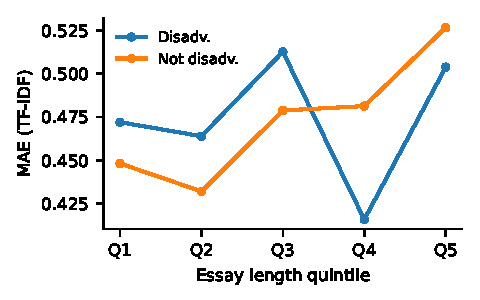
\includegraphics[width=0.48\linewidth]{figs/error_by_length.pdf}}{\pending{Error by length (\texttt{figs/error\_by\_length.pdf})}}
  \caption{Left: DeBERTa-v3 training and validation MSE with validation QWK. Right: test MAE by essay-length quintile and SES group.}
  \label{fig:curves}
\end{figure}

\begin{figure}[h]
  \centering
  \IfFileExists{figs/signed_error_by_score.pdf}{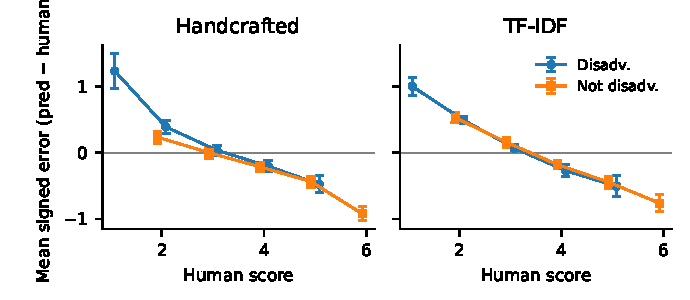
\includegraphics[width=0.75\linewidth]{figs/signed_error_by_score.pdf}}{\pending{Conditional signed error (\texttt{figs/signed\_error\_by\_score.pdf})}}
  \caption{Mean signed error by human score and SES group, with 95\% intervals; this is the conditional gap $\Delta_s$ from \cref{sec:method}. Points below zero are under-scored.}
  \label{fig:conditional}
\end{figure}

\paragraph{Results.} \TODO{After running the script, summarize \cref{tab:results} in 2--3 sentences: accuracy ranking of B1, B2, and DeBERTa; sign and CI of $\Delta$ for each; whether the neural model's gap is larger than the feature baselines'.}

\paragraph{Error analysis.} We examine (i) conditional errors (\cref{fig:conditional}), since all models are expected to over-predict at score~1 and under-predict at score~6 and the question is whether this compression differs by group; (ii) error by length (\cref{fig:curves}, right), because 512-token truncation removes the end of long essays, and essay length correlates with both score and SES; and (iii) the 50 largest test errors (\texttt{results/largest\_errors.csv}), which we read for systematic patterns such as off-prompt responses or heavy misspellings. \TODO{Add 2--3 sentences on what these show.}

\subsection{Ablation Study Plan}
\label{sec:ablation}

Each ablation varies one factor from the DeBERTa-v3 configuration above, with three seeds per setting.

\begin{table}[h]
  \centering
  \caption{Planned ablations. Each row changes a single component.}
  \label{tab:ablations}
  \small
  \begin{tabularx}{\linewidth}{l X X}
    \toprule
    Factor & Settings & Question answered \\
    \midrule
    Context length & 256 / 512 / long-context encoder & Does truncation drive the gap? (RQ2) \\
    Spelling & raw vs.\ spell-corrected input & Do mechanics carry the SES signal? (RQ2) \\
    Length control & full vs.\ length-matched test subsets & Is the gap a length artifact? (RQ2) \\
    Model size & DeBERTa-v3 small / base & Does capacity change bias? (RQ1) \\
    Prompt setting & prompt-specific vs.\ leave-one-prompt-out & Replicates \citet{yang2024tapestry} (RQ1) \\
    Mitigation & none / M1 ($\lambda \in \{0.1, 0.5, 1\}$) / M2 / M3 & Accuracy--fairness trade-off (RQ3) \\
    Probe & linear probe for $D$ on frozen embeddings & How much SES information is encoded? \\
    \bottomrule
  \end{tabularx}
\end{table}

% =====================================================================
\section{Next Steps}
\label{sec:next}

\begin{enumerate}
  \item Complete DeBERTa-v3 base runs with three seeds and report mean and standard deviation.
  \item Run the RQ2 input ablations (\cref{tab:ablations}) and the SES linear probe.
  \item Implement M1--M3 and plot the accuracy--fairness frontier across $\lambda$.
  \item Extend the analysis to the intersection of SES with English-learner status.
  \item Write the full report, with an ethics section on the limits of a binary SES flag and on deployment implications.
\end{enumerate}

% =====================================================================
\section{Member Contributions}
\label{sec:contrib}

\begin{table}[h]
  \centering
  \small
  \begin{tabularx}{\linewidth}{l X}
    \toprule
    Member & Responsibilities \\
    \midrule
    Carlos Canales & Project framing, data pipeline, fairness metrics, Overleaf and repository setup \\
    \TODO{Teammate 2} & \TODO{e.g., DeBERTa training and ablations} \\
    \TODO{Teammate 3} & \TODO{e.g., literature review, error analysis, mitigation methods} \\
    \bottomrule
  \end{tabularx}
\end{table}

\paragraph{Ethics.} PERSUADE is de-identified and released for research use. A binary eligibility flag is a coarse proxy for socioeconomic status, and group-level findings must not be read as statements about individual students.

\bibliographystyle{plainnat}
\bibliography{references}

\end{document}
